%%%%%%%%%%%%%%%%%%%%%%%%%%%%%%%%%%%%%%%%%%  不使用 authblk 包制作标题  %%%%%%%%%%%%%%%%%%%%%%%%%%%%%%%%%%%%%%%%%%%%%%
%-------------------------------PPT Title-------------------------------------
\title{密度泛函理论、\textrm{PAW}和\rm{VASP}概要}
%-----------------------------------------------------------------------------

%----------------------------Author & Date------------------------------------
\author[\textrm{Jun\_Jiang}]{姜\;\;骏\inst{}} %[]{} (optional, use only with lots of authors)
%% - Give the names in the same order as the appear in the paper.
%% - Use the \inst{?} command only if the authors have different
%%   affiliation.
\institute[BCC]{\inst{}%
%\institute[Gain~Strong]{\inst{}%
\vskip -20pt 北京市计算中心}
%\vskip -20pt {\large 格致斯创~科技}}
\date[\today] % (optional, should be abbreviation of conference name)
{	{\fontsize{6.2pt}{4.2pt}\selectfont{\textcolor{blue}{E-mail:~}\url{jiangjun@bcc.ac.cn}}}
\vskip 45 pt {\fontsize{8.2pt}{6.2pt}\selectfont{%清华大学\;\;物理系% 报告地点
	\vskip 5 pt \textrm{2022.12.16}}}
}

%% - Either use conference name or its abbreviation
%% - Not really information to the audience, more for people (including
%%   yourself) who are reading the slides onlin%%   yourself) who are reading the slides onlin%%   yourself) who are reading the slides onlineee
%%%%%%%%%%%%%%%%%%%%%%%%%%%%%%%%%%%%%%%%%%%%%%%%%%%%%%%%%%%%%%%%%%%%%%%%%%%%%%%%%%%%%%%%%%%%%%%%%%%%%%%%%%%%%%%%%%%%%

\subject{}
% This is only inserted into the PDF information catalog. Can be left
% out.
%\maketitle
\frame
{
%	\frametitle{\fontsize{9.5pt}{5.2pt}\selectfont{\textcolor{orange}{“高通量并发式材料计算算法与软件”年度检查}}}
\titlepage
}
%-----------------------------------------------------------------------------

%------------------------------------------------------------------------------列出全文 outline ---------------------------------------------------------------------------------
\section*{}
\frame[allowframebreaks]
{
  \frametitle{Outline}
%  \frametitle{\textcolor{mycolor}{\secname}}
  \tableofcontents%[current,currentsection,currentsubsection]
}
%%在每个section之前列出全部Outline
%%类似的在每个subsection之前列出全部Outline是\AtBeginSubsection[]
%\AtBeginSection[]
%{
%  \frame<handout:0>%[allowframebreaks]
%  {
%    \frametitle{Outline}
%%全部Outline中,本部分加亮
%    \tableofcontents[current,currentsection]
%  }
%}

%-----------------------------------------------PPT main Body------------------------------------------------------------------------------------
\small
\frame
{
	\frametitle{科学研究的范式变更}
\begin{figure}[h!]
\vspace*{0.08in}
\centering
\includegraphics[height=2.00in,width=4.15in]{Figures/Four_Model_3.png}
%\caption{\tiny \textrm{Pseudopotential for metallic sodium, based on the empty core model and screened by the Thomas-Fermi dielectric function.}}%(与文献\cite{EPJB33-47_2003}图1对比)
\label{Four_Model}
\end{figure}
}

\begin{frame}{科学研究的重要手段:~计算模拟}
\begin{figure}[h!]
\vspace*{-0.18in}
\centering
\includegraphics[height=2.55in,width=4.05in]{Figures/Schematic_Material-Design.png}
%\caption{\tiny \textrm{Pseudopotential for metallic sodium, based on the empty core model and screened by the Thomas-Fermi dielectric function.}}%(与文献\cite{EPJB33-47_2003}图1对比)
%\caption{\tiny \textrm{Pseudopotential for metallic sodium, based on the empty core model and screened by the Thomas-Fermi dielectric function.}}%(与文献\cite{EPJB33-47_2003}图1对比)
\label{Schematic_Material-Design}
\end{figure}
\end{frame}

\frame
{
	\frametitle{材料模拟的基本思想和方法}
\begin{figure}[h!]
\vspace*{-0.25in}
\centering
\includegraphics[height=0.80in,width=4.05in]{Figures/MGE-2.png}
%\caption{\tiny \textrm{Pseudopotential for metallic sodium, based on the empty core model and screened by the Thomas-Fermi dielectric function.}}%(与文献\cite{EPJB33-47_2003}图1对比)
\vskip 0.05pt
\includegraphics[height=2.20in,width=3.45in]{Figures/Multi-Scale-6.png}
%\caption{\tiny \textrm{Pseudopotential for metallic sodium, based on the empty core model and screened by the Thomas-Fermi dielectric function.}}%(与文献\cite{EPJB33-47_2003}图1对比)
\label{Multi-Scale}
\end{figure}
}

\begin{frame}
	\frametitle{理论、方法与软件}
\begin{figure}[h!]
\vspace*{-0.25in}
\centering
\includegraphics[height=2.80in,width=4.95in,viewport=5 3 1250 780,clip]{Figures/Method_Procedure.png}
%\caption{\tiny \textrm{Pseudopotential for metallic sodium, based on the empty core model and screened by the Thomas-Fermi dielectric function.}}%(与文献\cite{EPJB33-47_2003}图1对比)
\label{Method-Procedure}
\end{figure}
\end{frame}

\section{\rm{Density Functional Theory}}
\begin{frame}
	\frametitle{密度泛函理论}
	与传统的量子力学方法不同,密度泛函理论(\textrm{Density Functional Theory, DFT})的基本变量是体系的基态电子密度%
\begin{figure}[h!]
\vspace*{-0.18in}
\centering
\includegraphics[height=1.75in,width=4.05in]{Figures/Wavefun-Density.png}
\caption{\tiny \textrm{The wavefunction and density functional theory.}}%(与文献\cite{EPJB33-47_2003}图1对比)
\label{Wavefunction-Density}
\end{figure}
密度泛函理论的优越性:~用密度($\rho$)代替波函数($\Psi$)描述体系\\体系基态能量用粒子密度表示:~$E[\rho]$
\end{frame}

\frame                               %
{
\frametitle{\textrm{Kohn-Sham}方程}
\textrm{DFT}的基本方程是\textrm{Kohn-Sham}方程\upcite{PR136-B864_1964,PR140-A1133_1965}:~\\
将相互作用粒子替换成\textcolor{blue}{无相互作用粒子}\textcolor{red}{+}\textcolor{blue}{交换-相关能}的贡献
$$(T_S+V_{e\!f\!f})|\varphi_i\rangle=\varepsilon_i|\varphi_i\rangle,\quad i=1,\cdots,N,\cdots$$
其中$T_S=-\dfrac12\nabla^2$~~是无相互作用体系的动能
\begin{displaymath}
	\begin{aligned}
		V_{e\!f\!f}(\vec r)=&V_{ext}(\vec r)+\displaystyle\int w(\vec r,\vec r\,')\rho(\vec r\,')\mathrm{d}\vec r\,'+V_{\mathrm{XC}}[\rho]\\
=&\displaystyle\int\dfrac{\rho(\vec r\,')}{|\vec r-\vec r^{\prime}|}\mathrm{d}\vec r\,'+V_{ext}(\vec r)+V_{\mathrm{XC}}[\rho]
	\end{aligned}
\end{displaymath}
$V_{ext}(\vec r)$是电子体系与外部的电荷或磁场相互作用\\
$V_{\mathrm{XC}}[\rho]=\dfrac{\delta E_{\mathrm{XC}}}{\delta\rho(\vec r)}$称为交换-相关势
\vskip 10pt
%\textrm{Kohn-Sham}方程是形式上的单粒子方程
%\vskip 6pt
\textrm{Kohn-Sham}方程的实质:\\\textcolor{red}{将动能泛函的主要部分分离出来,剩余部分放在交换-相关能中}
}

\frame                               %
{
\frametitle{交换-相关能密度泛函}
\textcolor{blue}{密度泛函理论的核心问题}:\\
\textrm{Kohn-Sham}方程用于实际计算,必须知道$E_{XC}[\rho]$或者$V_{XC}[\rho]$与$\rho(\vec r)$的泛函关系
\vskip 15pt
\begin{minipage}[b]{0.59\textwidth}
 \hspace*{-15pt}
 {\fontsize{7.5pt}{6.0pt}\selectfont\begin{itemize}%[+-| alert@+>]
	 \setlength{\itemsep}{10pt}
 \item \textrm{LDA}:泛函只与密度分布的局域值有关
 \item \textrm{GGA}:泛函依赖:局域密度及其梯度
 \item $meta$-\textrm{GGA}:泛函依赖的变量还有动能密度
 \item 杂化(\textrm{hybrid})泛函:泛函与占据轨道有关
 \item 其他的交换-相关能泛函
 \item<1-> 完全非局域泛函:理想泛函,不现实
 \end{itemize}}
\end{minipage}
\hfill
\begin{minipage}[b]{0.39\textwidth}
\hspace*{-10pt}
\includegraphics[height=1.7in,width=3.18in,viewport=10 5 1380 700,clip]{Figures/Jacobi-ladder.png}\\
\centering{\textcolor{red}{\textrm{\tiny Jacob's ladder}}}
\end{minipage}
% \begin{itemize}%[+-| alert@+>]
%\item 交换-相关能密度泛函
}

\frame                               %
{
	\frametitle{\textrm{Kohn-Sham}方程}
\begin{figure}[h!]
\centering
\vspace*{-0.21in}
\hspace*{-0.1in}
\includegraphics[height=2.4in,width=3.6in,viewport=2 5 1162 880,clip]{Figures/DFT.png}
\caption{\tiny \textrm{The Analysis of Kohn-Sham equation.}}%(与文献\cite{EPJB33-47_2003}图1对比)
\label{DFT}
\end{figure}
各种方法的\textcolor{red}{主要区别}:~\textcolor{blue}{势函数的处理}与\textcolor{blue}{所选基函数类型}不同
}

\frame
{
	\frametitle{\textrm{DFT}-\textit{SCF}}
\begin{figure}[h!]
\centering
\vspace*{-0.32in}
\hspace*{-0.80in}
\includegraphics[height=2.80in,width=4.95in,viewport=5 3 1490 870,clip]{Figures/DFT-SCF_2.png}
%\caption{\tiny \textrm{Pseudopotential for metallic sodium, based on the empty core model and screened by the Thomas-Fermi dielectric function.}}%(与文献\cite{EPJB33-47_2003}图1对比)
\label{DFT-SCF-2}
\end{figure}
}

\section{\rm{PAW}方法}
\frame
{
%	\frametitle{\textrm{PAW}原子数据集}
	\frametitle{\textrm{PAW Augmentation}}
\begin{figure}[h!]
\centering
\includegraphics[height=2.3in,width=4.0in,viewport=0 0 1280 745,clip]{Figures/PAW-baseset.png}
\caption{\tiny \textrm{The Augmentation of PAW.}}%(与文献\cite{EPJB33-47_2003}图1对比)
\label{PAW_baseset}
\end{figure}
}

\frame
{
	\frametitle{\textrm{PAW}方法的基组和势}
\begin{figure}[h!]
\centering
\includegraphics[height=1.0in,width=4.1in,clip]{Figures/Pseudo-Potential.png}
\caption{\tiny \textrm{The relation of Pseudo potential and PAW.}}%(与文献\cite{EPJB33-47_2003}图1对比)
\label{Pseudo_Potential_PAW}
\end{figure}
}

\section{\rm{VASP}软件}
\frame
{
	\frametitle{\textrm{VASP}软件简介}
	\textrm{VASP}软件是维也纳大学\textrm{(Universit\"at Wien)}~\textrm{G. Kresse}等开发的第一原理模拟软件包
	\begin{itemize}
		\item \textrm{VASP}采用\textrm{PAW~(Projector Augmented-Wave)}方法\upcite{PRB50-17953_1994,PRB59-1758_1999},平衡了赝势方法和全电子计算优点,兼顾了计算的精度和效率
		\item \textrm{VASP}在实空间优化投影函数\textrm{(Projector)},将主要的计算过程变换到实空间完成,大大节省了内存的开销%,保证了计算精度和效率
		\item \textrm{VASP}通过引入多样的优化算法,提高了矩阵对角化和电荷密度搜索的效率
		\item 在\textrm{VASP}的并行计算中,有效均衡了各节点处理\textrm{FFT}变换负载和通信,提升了软件的并行效率
	\end{itemize}
	相比于其他第一原理计算软件,\textrm{VASP}从物理思想与方法、优化算法和并行计算实现等多个方面都有更为出色的性能
}

\frame
{
	\frametitle{\textrm{VASP}的开发团队}
\begin{figure}[h!]
\centering
\vspace*{-0.25in}
\includegraphics[height=2.70in,width=4.05in,viewport=330 130 1280 770,clip]{Figures/VASP_team.png}
\caption{\tiny \textrm{The development team of VASP.}}%(与文献\cite{EPJB33-47_2003}图1对比)
\label{VASP_team}
\end{figure}
}

\frame
{
	\frametitle{\textrm{VASP}的\textrm{Kohn-Sham}方程求解流程}
\begin{figure}[h!]
	\vspace{-0.2in}
\centering
%\includegraphics[height=2.7in,width=4.0in,viewport=0 0 1300 960,clip]{Figures/VASP_procedure-full.png}
%\includegraphics[height=2.1in,width=1.6in,viewport=0 0 480 630,clip]{Figures/VASP_procedure.png}
%\includegraphics[height=2.1in,width=2.3in,viewport=0 0 740 600,clip]{Figures/Ab-initio-Ene.png}
\includegraphics[height=2.75in,width=2.5in,viewport=0 0 480 630,clip]{Figures/VASP_procedure.png}
\caption{\tiny \textrm{The Flow of calculation for the KS-ground states.}}%(与文献\cite{EPJB33-47_2003}图1对比)
\label{PAW_baiseset}
\end{figure} 
}

\frame
{
	\frametitle{\textrm{VASP}的迭代收敛}
完整的\textrm{VASP}计算流程是离子-电子的耦合自洽迭代,称为从头算分子动力学\textrm{(Ab Initio Molecular Dynamics, AIMD)}
\vskip 3pt
	{\fontsize{6.2pt}{4.2pt}\selectfont{
		\begin{itemize}
		\item \textrm{AIMD}通过在动力学系统中引入经典力学的绝热能量,将\textrm{DFT}与\textrm{MD}关联起来,实现电子与离子运动在同一动力学框架内处理,同时又在时间尺度上保持分离
		\item \textrm{AIMD}框架下,\textrm{DFT}到\textrm{MD}跨尺度无需再借助势函数模拟,电子弛豫过程与分子动力学可以用类似的迭代方式计算,大大降低了程序的复杂度
	\end{itemize} }}
\begin{figure}[h!]
	\vspace{-0.2in}
\centering
%\includegraphics[height=2.7in,width=4.0in,viewport=0 0 1300 960,clip]{Figures/VASP_procedure-full.png}
\includegraphics[height=1.8in,width=2.6in,viewport=0 0 740 600,clip]{Figures/Ab-initio-Ene.png}
\caption{\tiny \textrm{The Flow of calculation for the AIMD.}}%(与文献\cite{EPJB33-47_2003}图1对比)
\label{PAW_AIMD}
\end{figure} 
}

\frame
{
	\frametitle{\textrm{VASP}的优化与迭代收敛}
	\textrm{VASP}计算中,资源消耗的主要部分是求解\textrm{Kohn-Sham}方程,即偏微分方程\textrm{(Partial Differential Equations,~PDE)}的自洽迭代, 迭代过程主要包括
	\begin{itemize}
		\item 矩阵的迭代对角化
		\item 电荷密度的自洽迭代
	\end{itemize}

	\vskip 10pt
	\textrm{VASP}的计算高效得益于求解过程中中应用了多种经典优化算法,保证了迭代计算的快速收敛
	\begin{itemize} 
		\item 拟牛顿法\textrm{(Quasi-Newton method)}
		\item 共轭梯度法\textrm{(Conjugate Gradients method, CG)}
		\item 残差最小化\textrm{(RMM-DIIS)}方法
	\end{itemize}
}

\frame
{
	\frametitle{\textrm{VASP}的并行效率}
	与同类型软件相比,\textrm{VASP}有着优异的并行能力
\begin{figure}[h!]
	\vspace{-0.15in}
\centering
%\includegraphics[height=2.7in,width=4.0in,viewport=0 0 1180 875,clip]{Figures/dual_grid.png}
\includegraphics[height=1.55in,width=1.95in,viewport=0 0 240 200,clip]{Figures/VASP-abinit_Li128-1.png}
\includegraphics[height=1.55in,width=1.95in,viewport=0 0 240 200,clip]{Figures/VASP-abinit_Li128-2.png}
\caption{\tiny \textrm{The comparison of parallel scaling for ABINIT vs VASP.}}%(与文献\cite{EPJB33-47_2003}图1对比)
\label{ABINIT_vs_VASP}
\end{figure} 
\begin{itemize}
	\item \textrm{VASP}迭代对角化约束了矩阵的维度,减少了对角化过程中的迭代次数,保证了\textrm{MPI}并行的规模和扩展性
	\item \textrm{VASP}实施\textrm{FFT}变换时,保证各节点上处理的网格负载均衡
\end{itemize}
}

\frame
{
	\frametitle{双网格技术}
\begin{figure}[h!]
	\vspace{-0.15in}
\centering
%\includegraphics[height=2.7in,width=4.0in,viewport=0 0 1180 875,clip]{Figures/dual_grid.png}
\includegraphics[height=2.75in,width=4.0in,viewport=0 0 800 600,clip]{Figures/dual_grid-2.png}
\caption{\tiny \textrm{The Schematic description of the dual grid technique.}}%(与文献\cite{EPJB33-47_2003}图1对比)
\label{PAW_dualgrid}
\end{figure} 
}

\frame
{
	\frametitle{\textrm{VASP}计算的\textrm{FFT}并行实现}
	\begin{itemize}
	     \item 中间层设计:~\textrm{FFT}网格、实空间基组与计算节点的匹配\\
		     \textcolor{red}{通过子程序\textrm{mgrid.F}生成中间层,实现并行负载与计算节点分配的匹配,减少\textrm{FFT}变换和实空间并行的节点间通信}
\begin{figure}[h!]
		\vspace{-0.25in}
	\centering
%\includegraphics[height=2.7in,width=4.0in,viewport=0 0 1180 875,clip]{Figures/dual_grid.png}
\includegraphics[height=1.0in,width=4.0in,viewport=0 0 1500 450,clip]{Figures/VASP_FFT-MPI_Reciprocal.png}
\vskip 0.5pt
\includegraphics[height=0.7in,width=4.0in,viewport=0 0 730 150,clip]{Figures/VASP_FFT-MPI_Real.png}
\caption{\tiny \textrm{VASP:~ Reciprocal-Real space layout for grids in MPI.}}%(与文献\cite{EPJB33-47_2003}图1对比)
\label{MPI-FFT}
\end{figure} 
	\end{itemize}
}

\frame
{
	\frametitle{\textrm{VASP}的通信开销}
	在高性能的计算队列中,\textrm{VASP}的并行上限可以突破256核,但当并行核数超过百核数量级,并行效率下降非常明显
\begin{figure}[h!]
	\vspace{-0.15in}
\centering
%\includegraphics[height=2.7in,width=4.0in,viewport=0 0 1180 875,clip]{Figures/dual_grid.png}
\includegraphics[height=1.55in,width=1.95in,viewport=0 0 240 200,clip]{Figures/VASP-mpi-Li128.png}
\caption{\tiny \textrm{Time spent in MPI calls with increasing the number of ranks in a VASP calculation.}}%(与文献\cite{EPJB33-47_2003}图1对比)
\label{VASP_communication}
\end{figure} 

如能对并行系统与\textrm{VASP}结合作深度改造(如国家超算天津中心方案),\textrm{VASP}的并行扩展可以到$10^4$核级别,但这一改造需要对底层代码和计算框架作较大规模改动
}

\frame
{
	\frametitle{\textrm{VASP}的\textrm{GPU}加速}
\textrm{NVIDIA}多年来致力于\textrm{VASP}的\textrm{GPU}加速,取得了一定的成效
\begin{figure}[h!]
	\vspace{-0.15in}
\centering
%\includegraphics[height=2.7in,width=4.0in,viewport=0 0 1180 875,clip]{Figures/dual_grid.png}
\includegraphics[height=1.2in,width=4.05in,viewport=0 0 850 260,clip]{Figures/VASP-GPU-CPU.png}
\caption{\tiny \textrm{Compare of VASP calculation with GPU and CPU.}}%(与文献\cite{EPJB33-47_2003}图1对比)
\label{VASP_GPU}
\end{figure} 
\begin{itemize}
	\item 通用配置下,\textrm{GPU}对\textrm{VASP}计算有加速效果,一般可提升4$\sim$6倍
	\item 矩阵对角化的并行算法限制了\textrm{GPU}在第一原理计算中的应用
	\item \textrm{GPU}加速的模式主要适合于分子动力学计算
\end{itemize}
}

%\frame[allowframebreaks]
\begin{frame}[allowframebreaks]{\textrm{VASP}的主程序结构}
\begin{figure}[h!]
\vskip -10pt
\centering
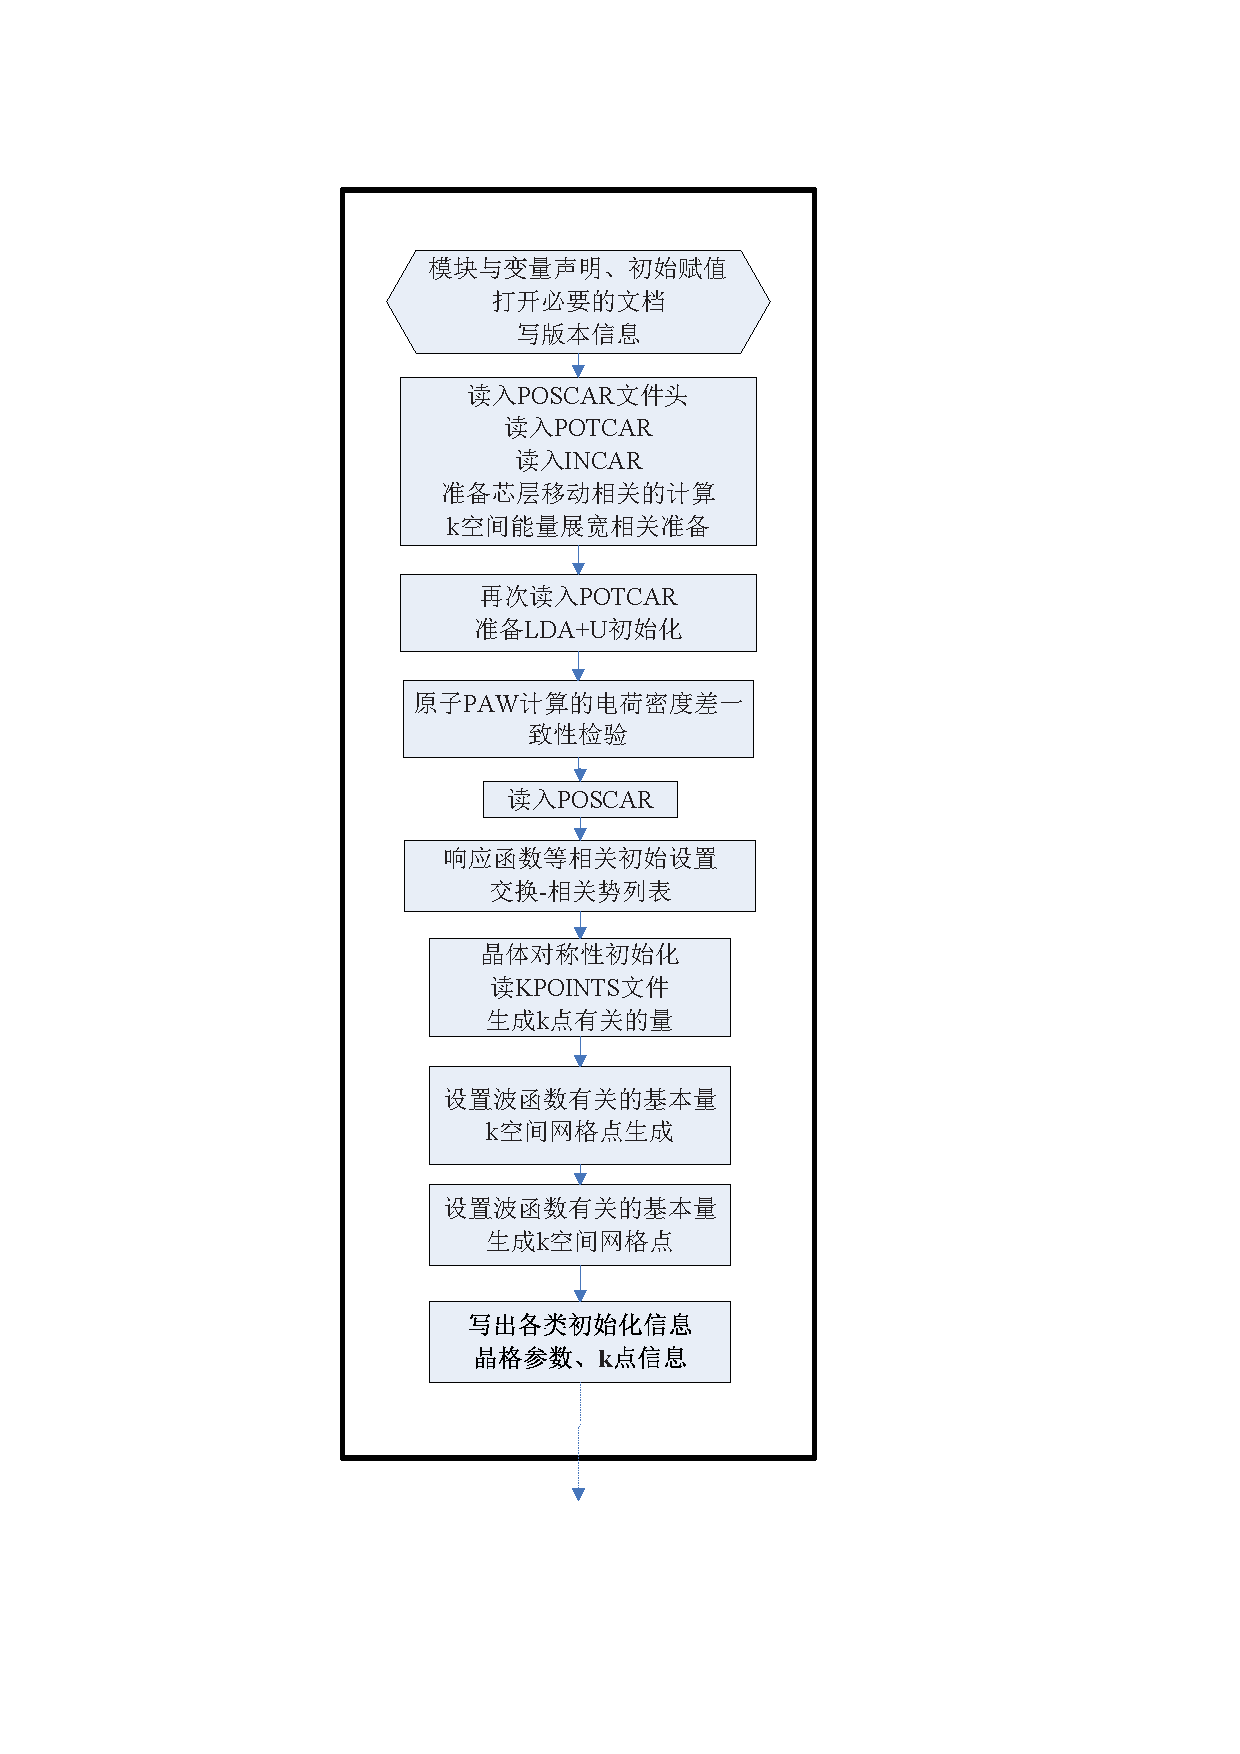
\includegraphics[height=2.65in,width=4.0in,viewport=0 360 562 720,clip]{Figures/VASP_main_Flow-1.png}
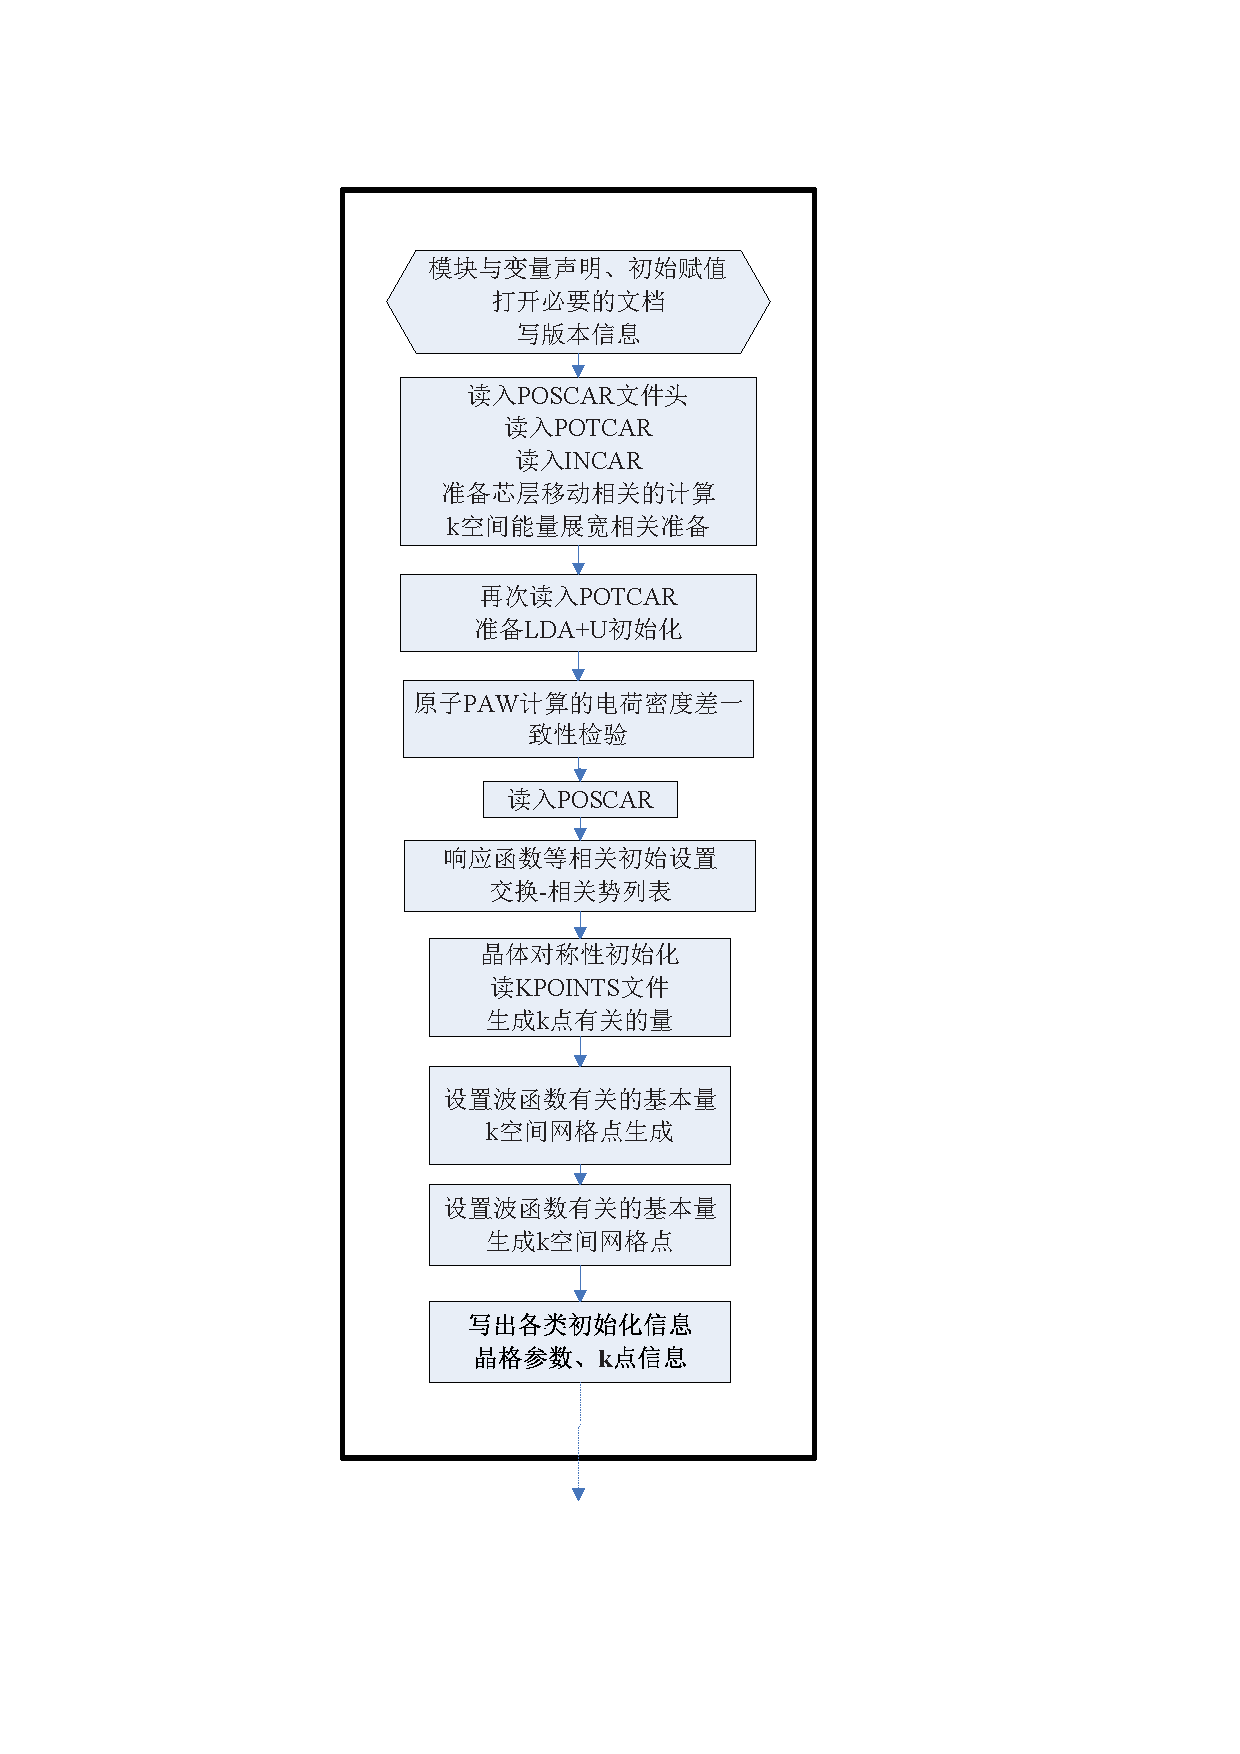
\includegraphics[height=2.65in,width=4.0in,viewport=0 0 562 360,clip]{Figures/VASP_main_Flow-1.png}
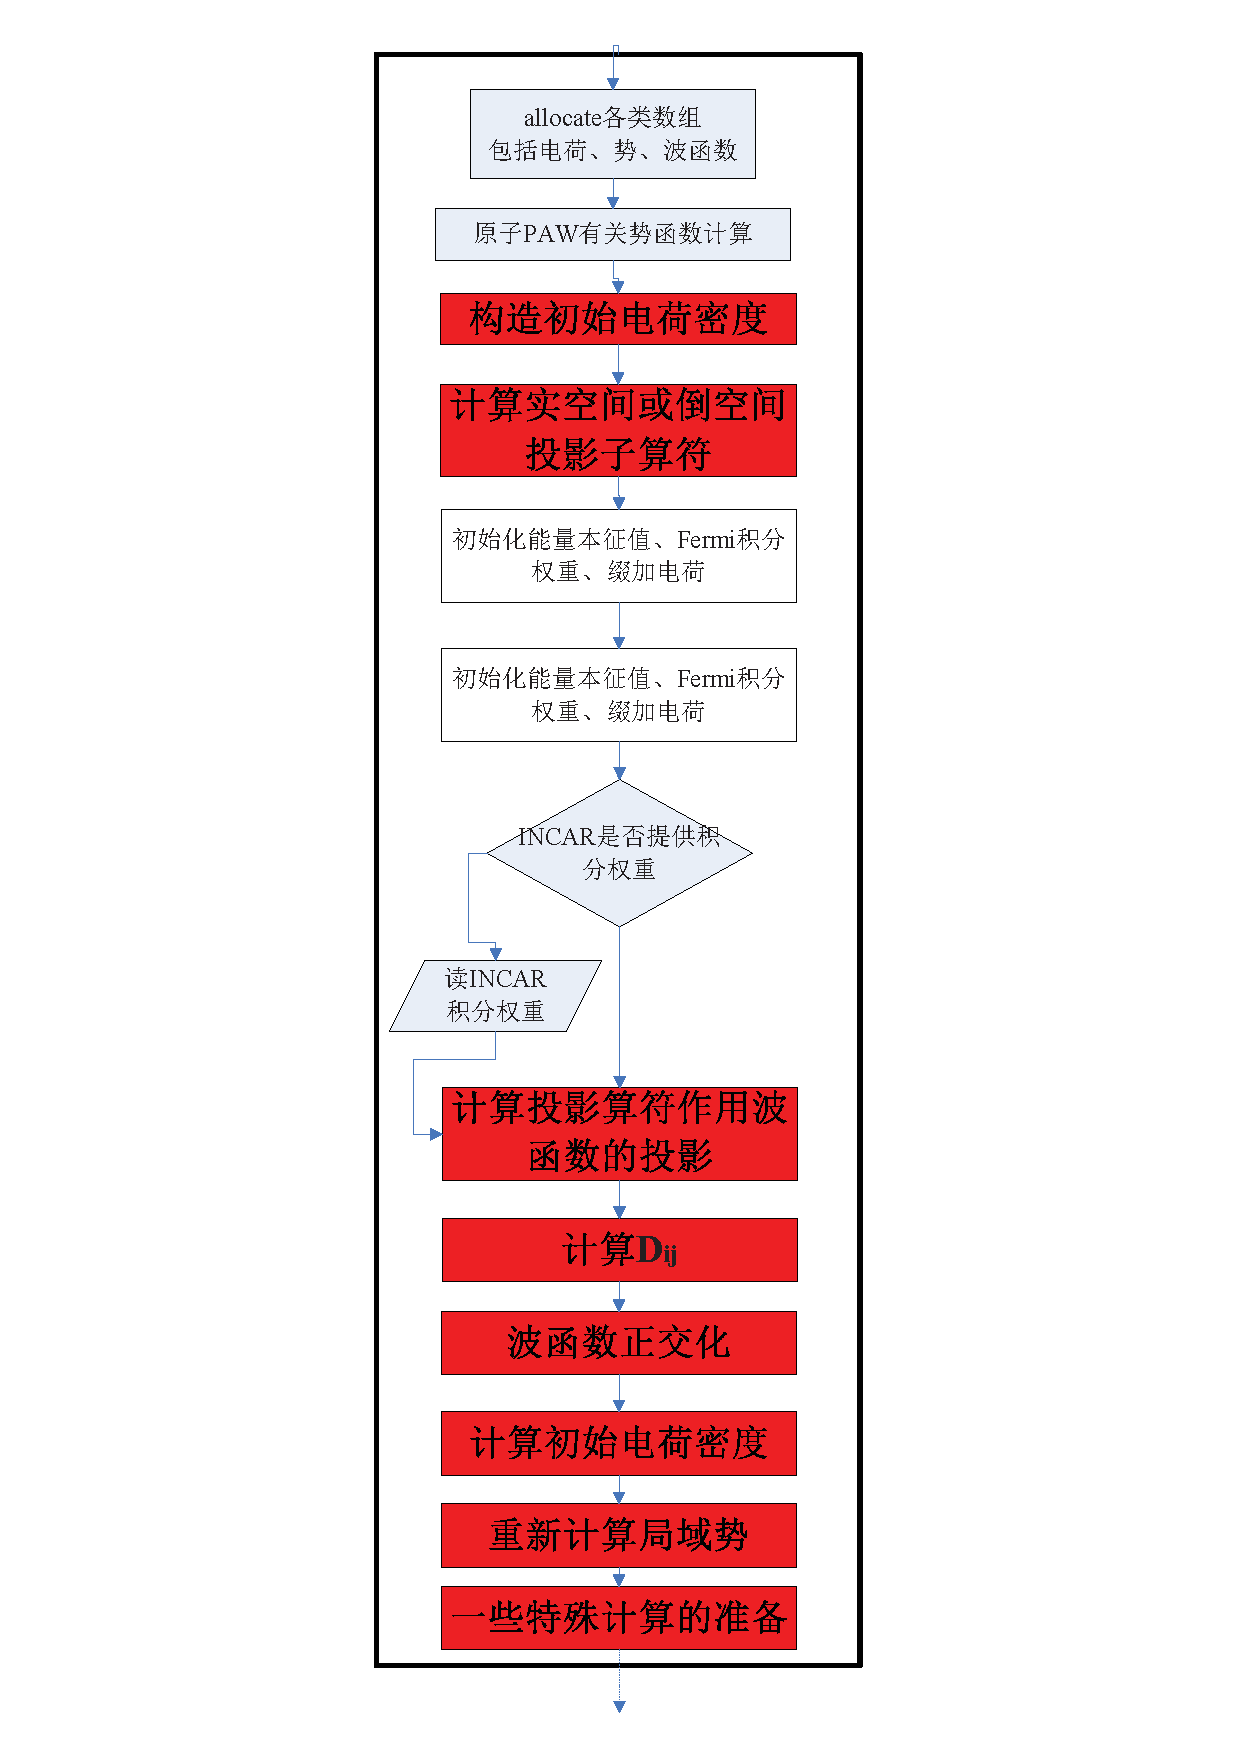
\includegraphics[height=2.35in,width=4.0in,viewport=0 370 562 680,clip]{Figures/VASP_main_Flow-2.png}
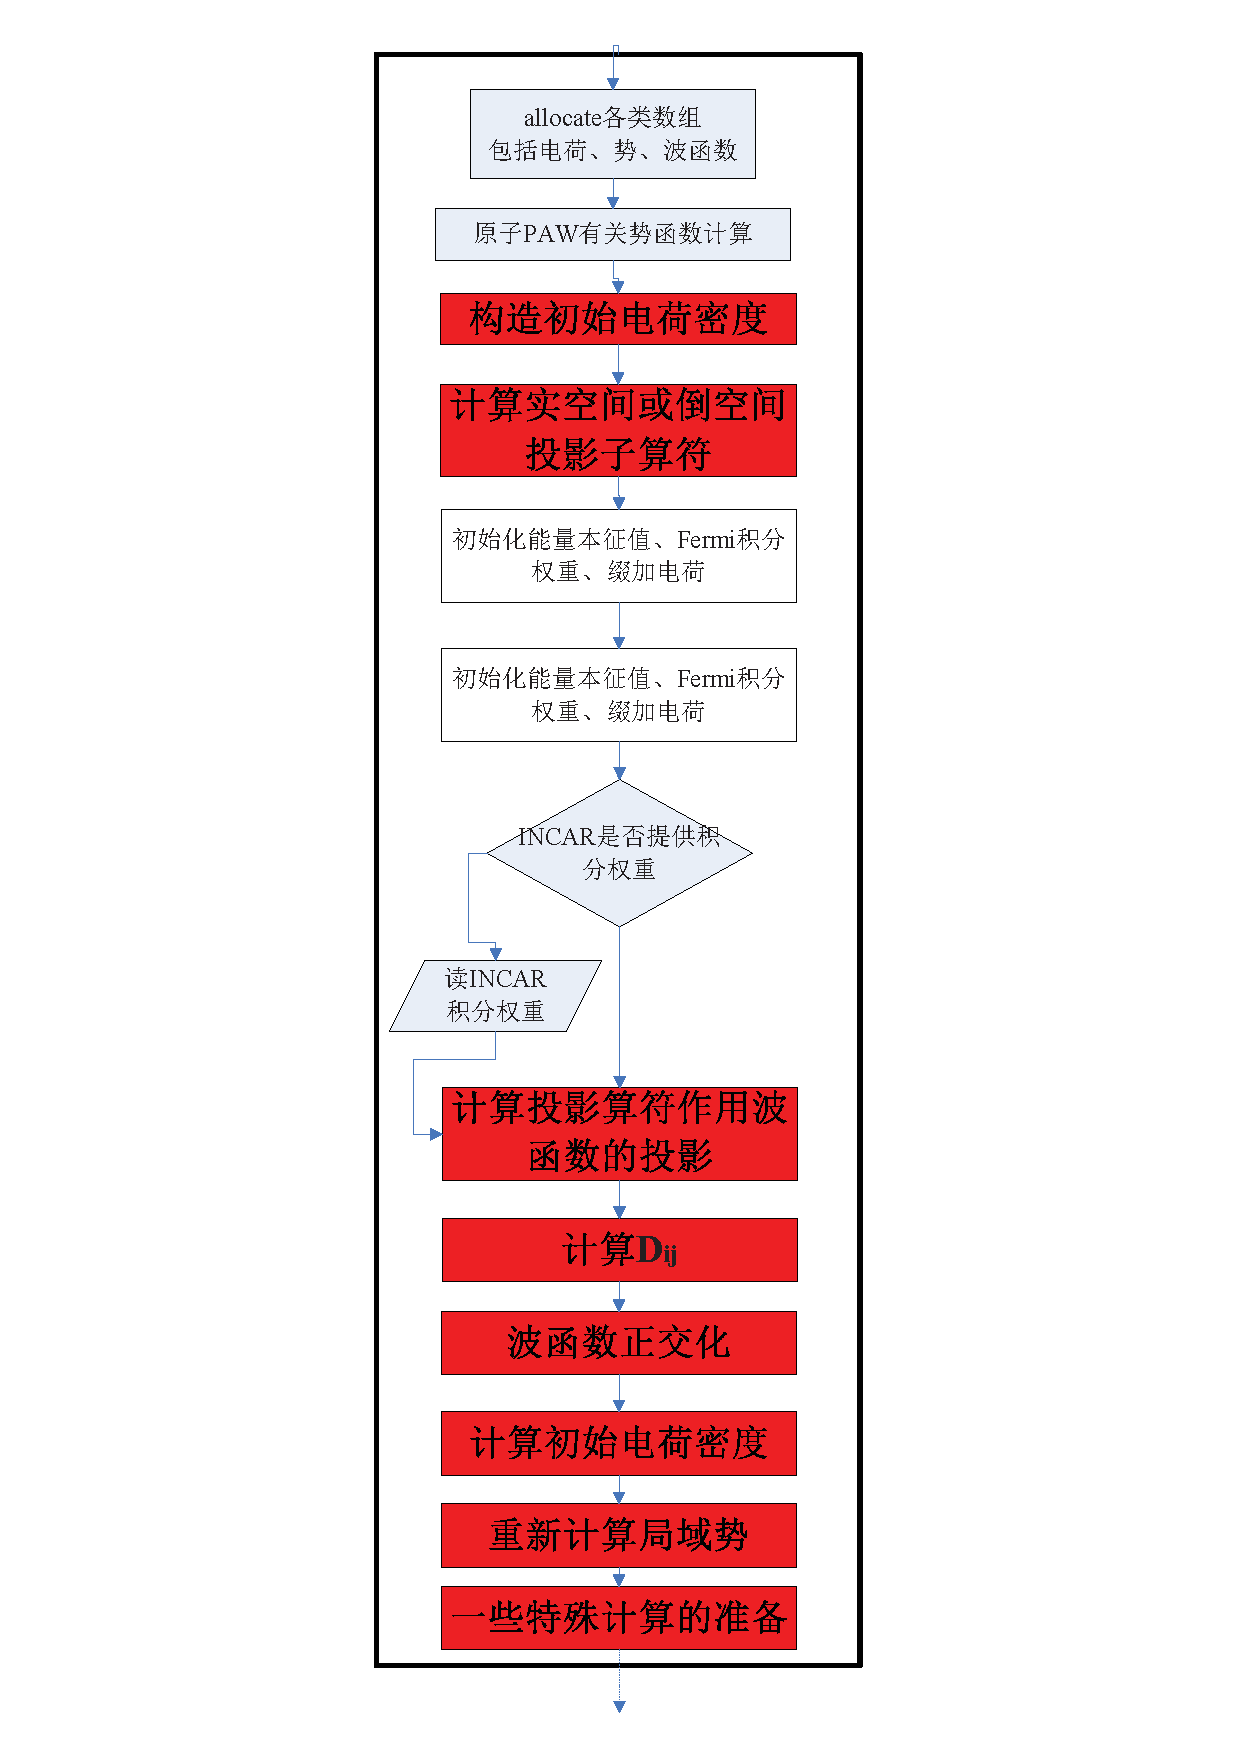
\includegraphics[height=2.50in,width=4.0in,viewport=0 0 562 370,clip]{Figures/VASP_main_Flow-2.png}
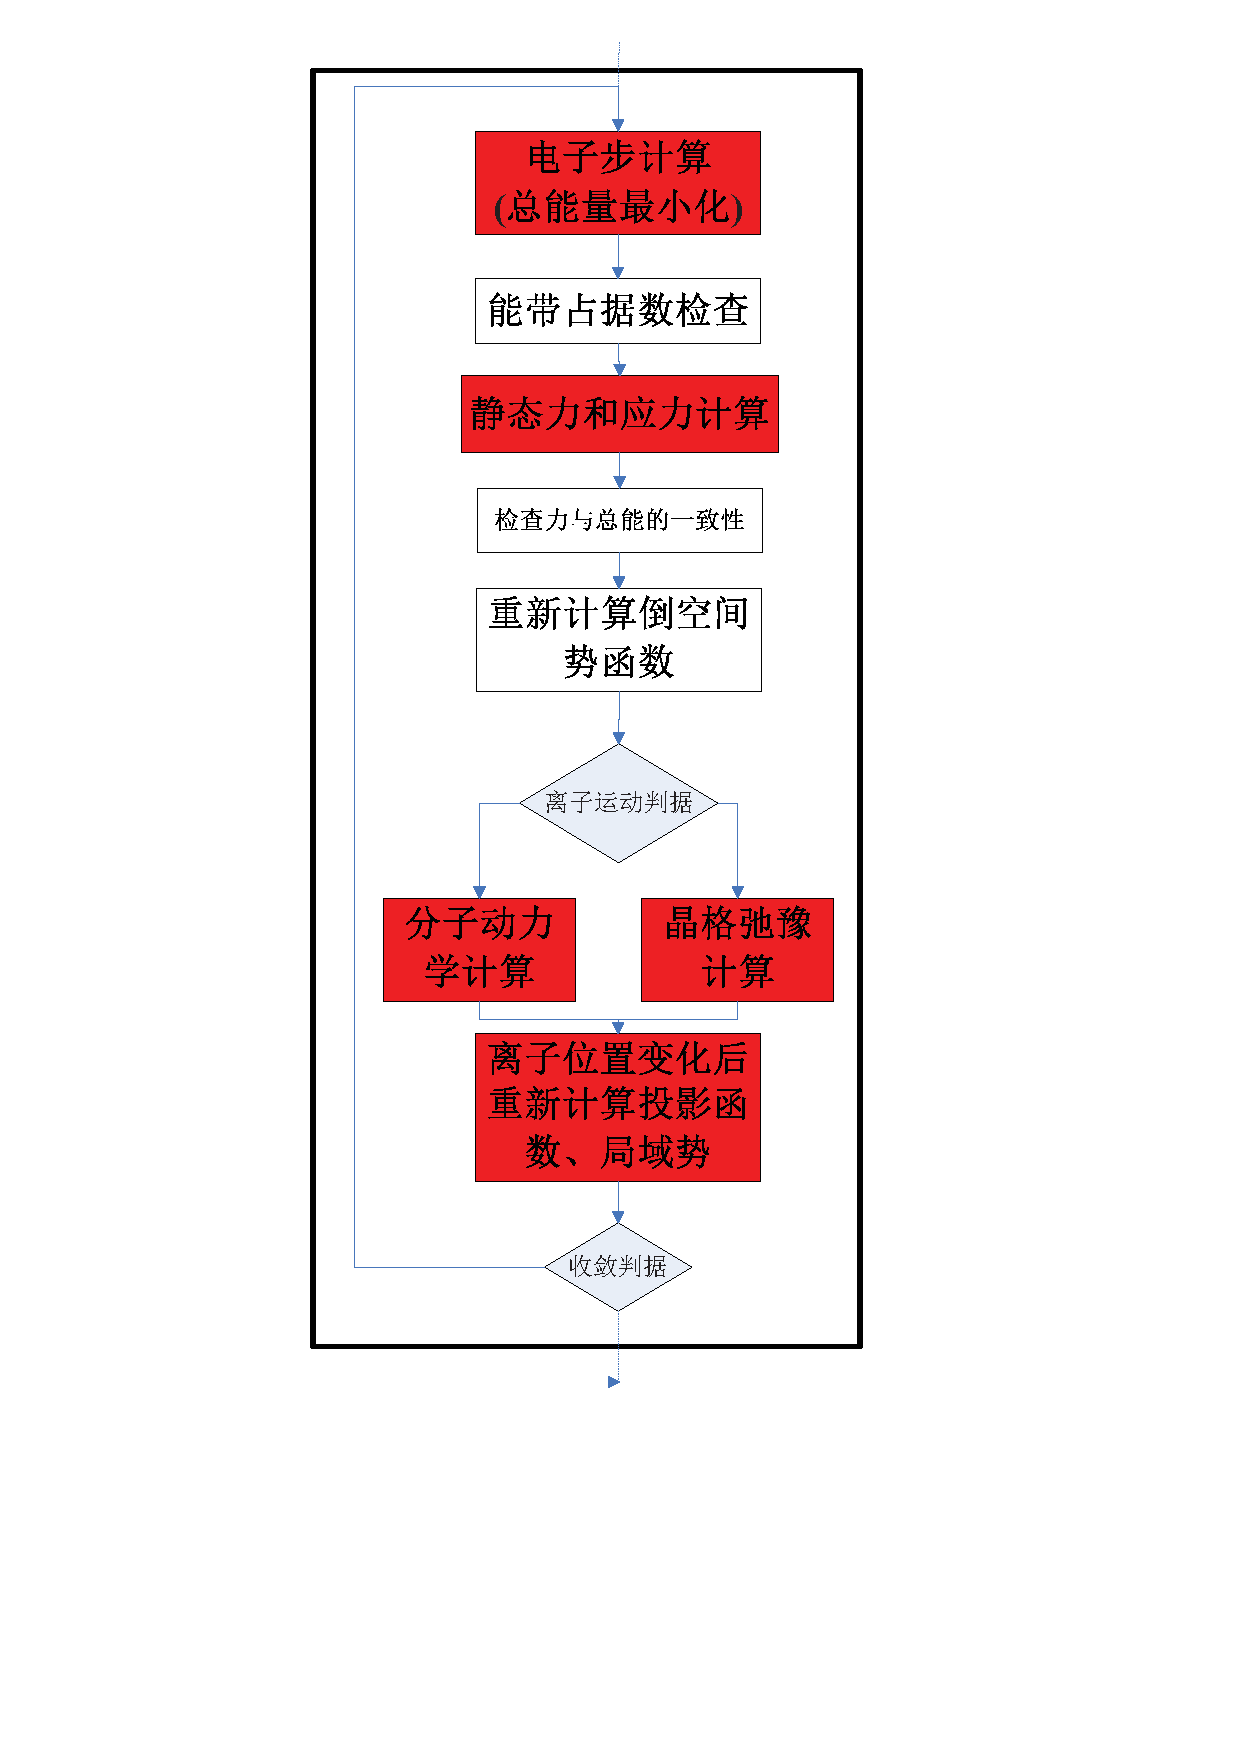
\includegraphics[height=2.45in,width=4.0in,viewport=0 350 562 660,clip]{Figures/VASP_main_Flow-3.png}
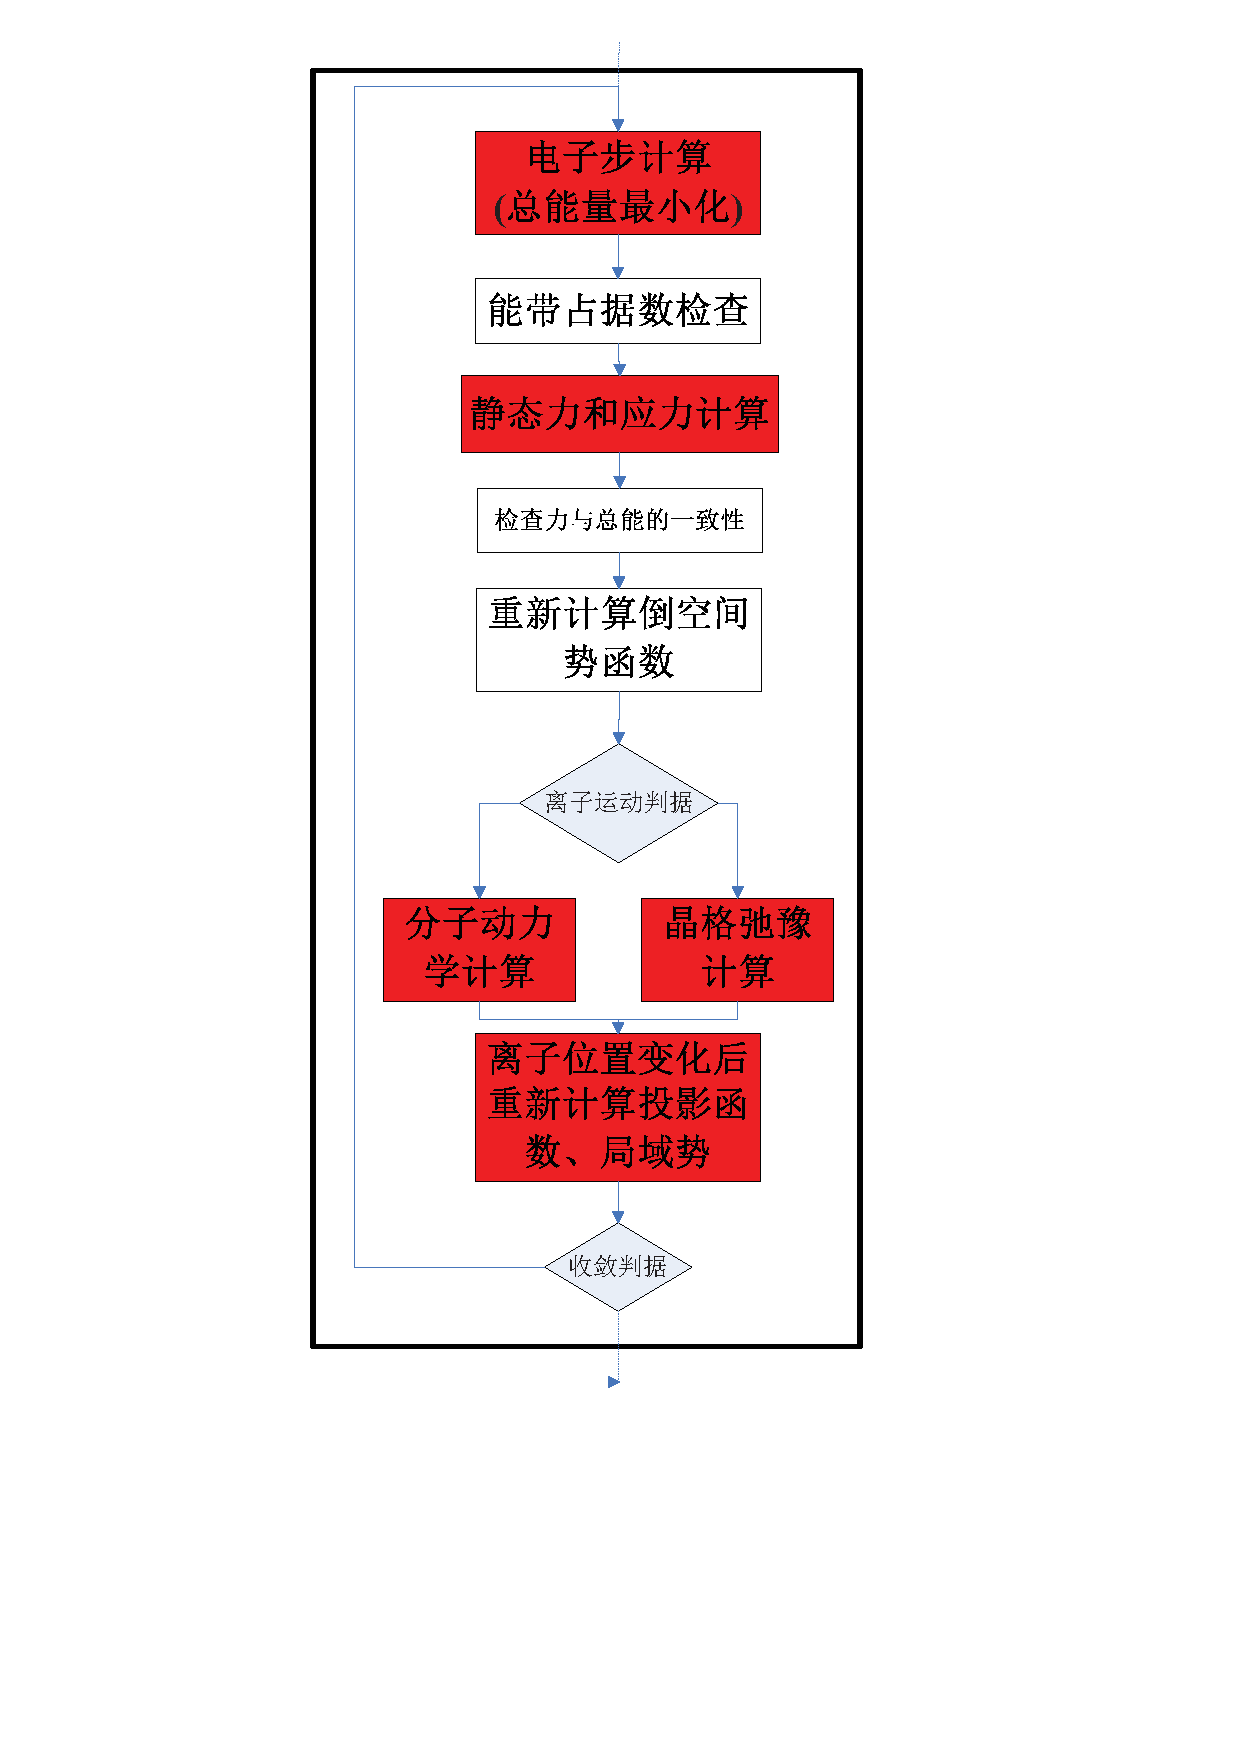
\includegraphics[height=2.50in,width=4.0in,viewport=0 0 562 350,clip]{Figures/VASP_main_Flow-3.png}
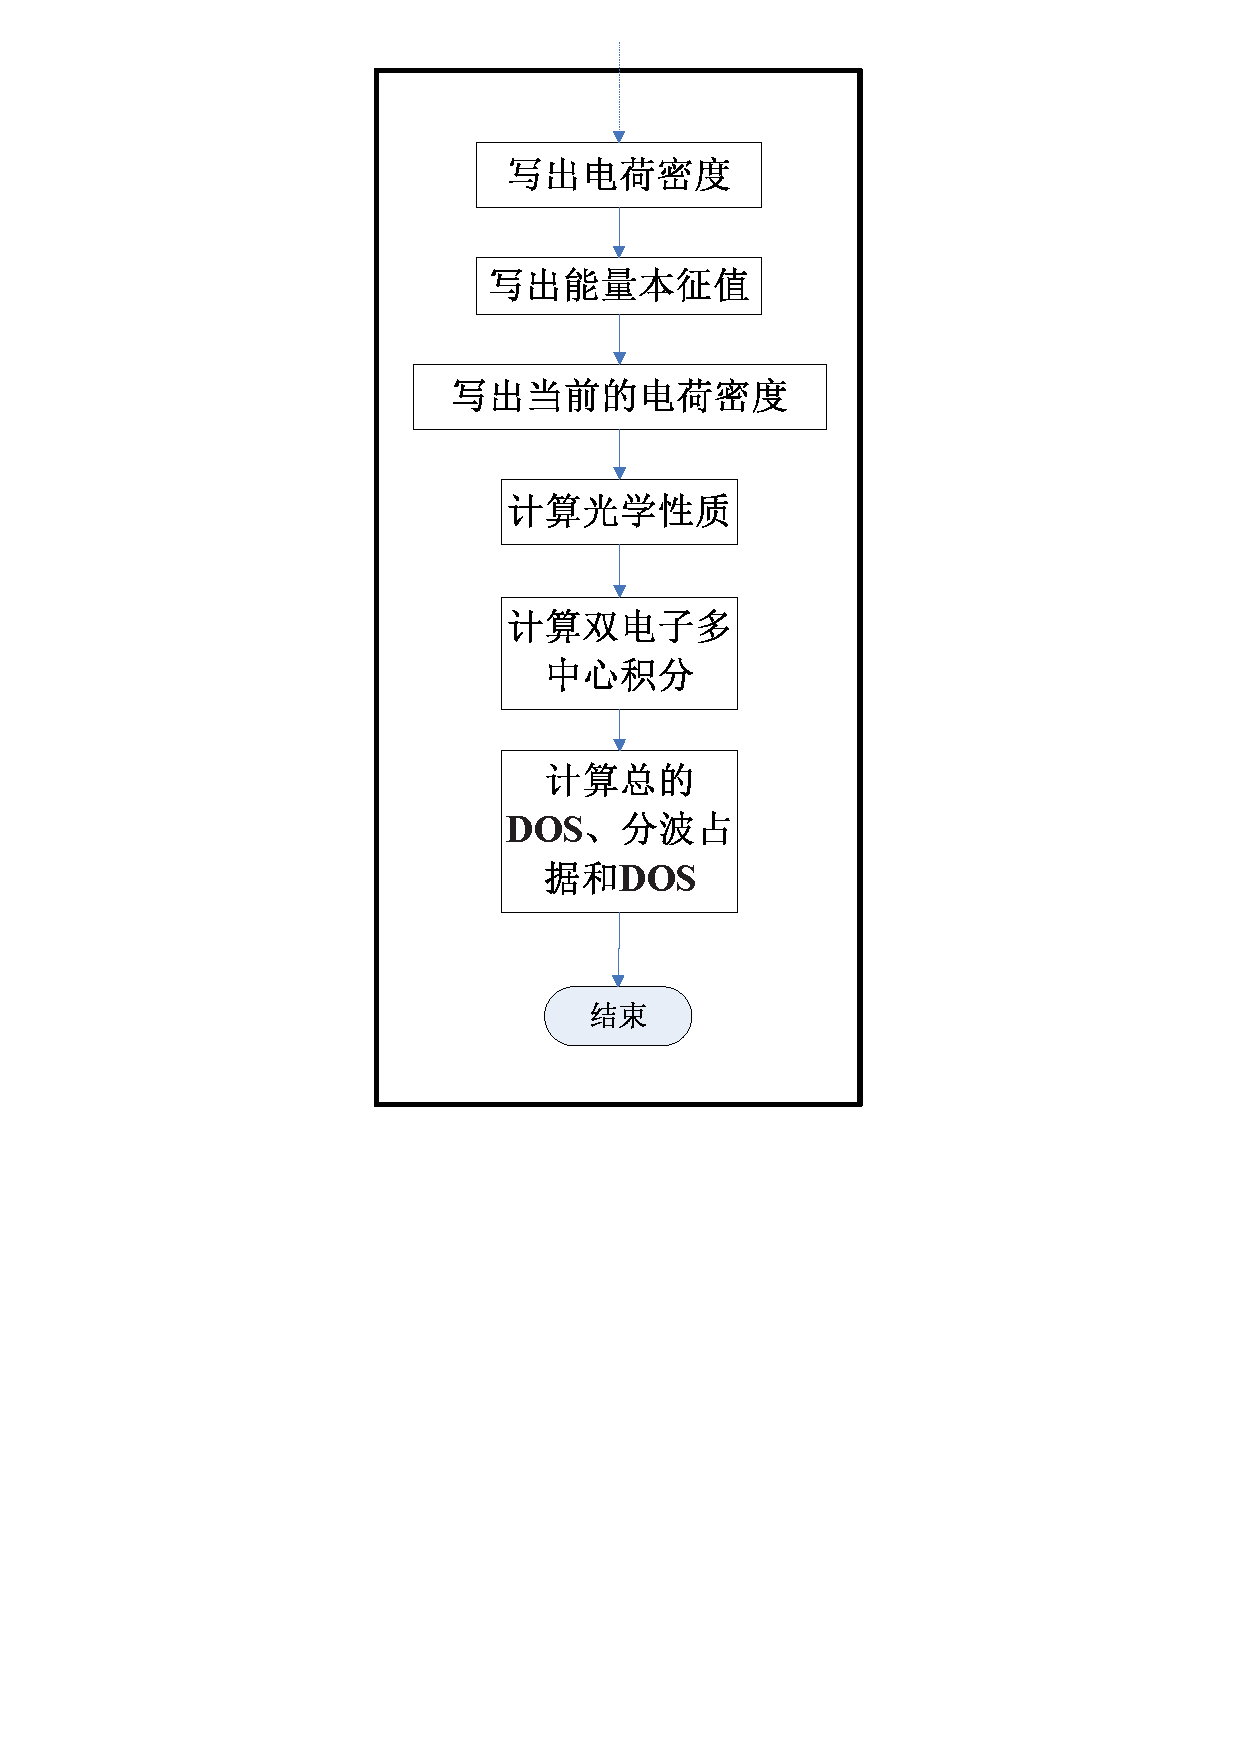
\includegraphics[height=2.30in,width=4.0in,viewport=0 215 562 530,clip]{Figures/VASP_main_Flow-4.png}
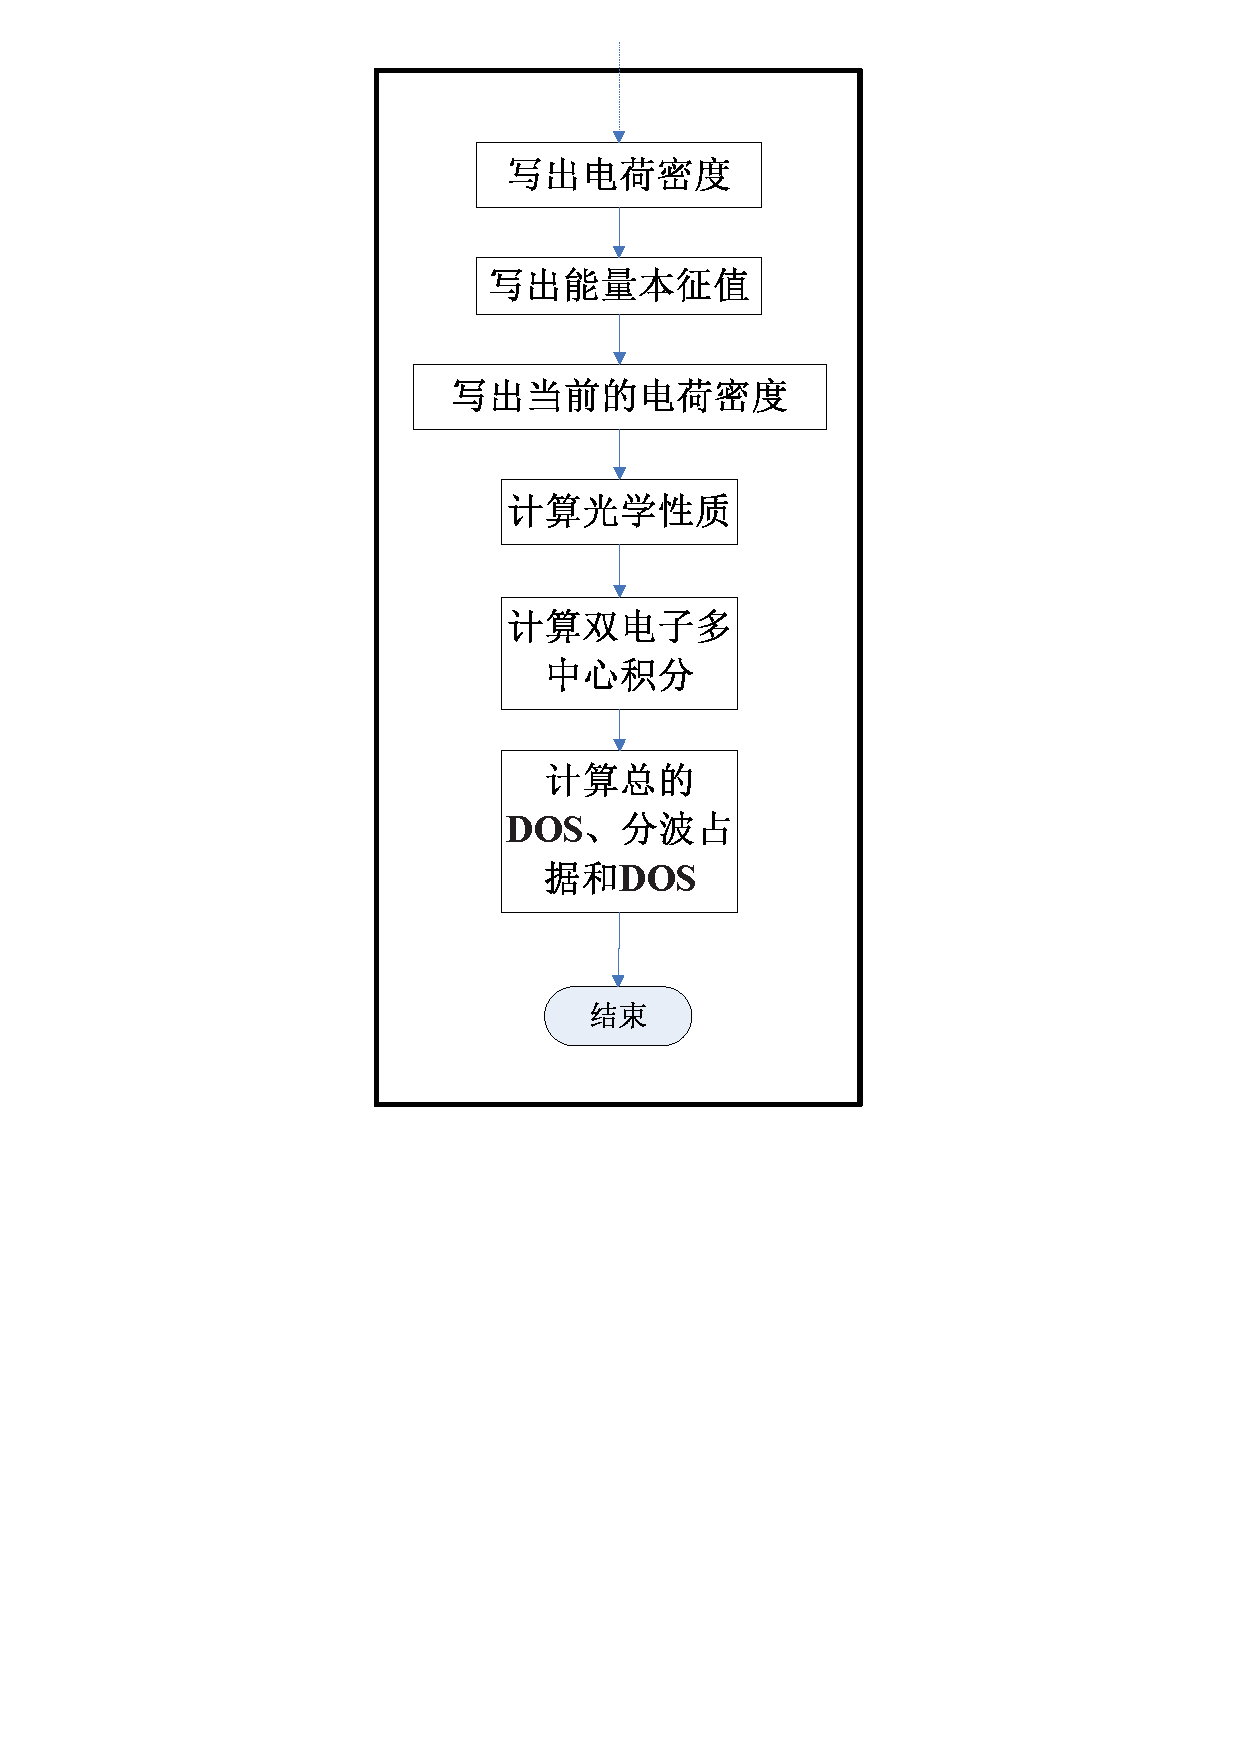
\includegraphics[height=1.40in,width=4.0in,viewport=0 0 562 215,clip]{Figures/VASP_main_Flow-4.png}
\caption{\tiny \textrm{The Flow of main program for VASP.}}%(与文献\cite{EPJB33-47_2003}图1对比)
\label{FLOW_of_VASP}
\end{figure}
\end{frame}

\section{小结}
\frame
{
	\frametitle{小结}
	作为第一性原理计算的商用软件,\textrm{VASP}已成为计算材料学领域应用最广泛的软件之一。全球绝大多数超算中心都安装了\textrm{VASP},据统计,\textrm{VASP}软件的作业机时占用全球总机时的12$\sim$20\%,但由于其%类似于linpack软件,
属于重型浮点计算密集型应用,实际耗电量占比则高达30$\sim$50\%
\vskip 3pt
	{\fontsize{9.0pt}{7.2pt}\selectfont{
	\begin{itemize}
		\item \textcolor{blue}{物理上},\textrm{VASP}基于\textrm{DFT}近似,求解\textrm{Kohn-Sham}方程,并将粒子基态密度问题转化为矩阵的本征函数和本征值问题
		\item \textcolor{blue}{数学上},方程求解过程的核心是矩阵对角化与\textrm{PDE}的自洽迭代,即便对于简单体系,也需要完成数十次的迭代,而规模大的计算模拟体系则可能需要成千上万次迭代计算
		\item \textcolor{blue}{计算过程上},\textrm{VASP}计算的时长开销主要是本征值求解的矩阵对角化;此外由于算法限制,\textrm{Kohn-Sham}方程作为线性方程组作并行处理时,节点间存在密集的通信。在上千节点,上万计算核的大规模并行系统上,数据通信将严重影响程序的性能,这是当前\textrm{VASP}软件的主要瓶颈
	\end{itemize}}}
			\textcolor{magenta}{有必要探索新的并行和优化策略来提升\textrm{VASP}的计算性能}
}

%------------------------------------------------------------------------Reference----------------------------------------------------------------------------------------------
		\frame[allowframebreaks]
{
\frametitle{主要参考文献}
\begin{thebibliography}{99}
{\tiny
	\bibitem{PR136-B864_1964}\textrm{P. Hohenberg and W. Kohn, \textit{Phys. Rev.} \textbf{136} (1964), B864}
	\bibitem{PR140-A1133_1965}\textrm{W. Kohn and L.J. Sham, \textit{Phys. Rev.} \textbf{140} (1965), A1133}
	\bibitem{PRB50-17953_1994}\textrm{P. E. Bl\"ochl. \textit{Phys. Rev.} B, \textbf{50} (1994), 17953}
	\bibitem{PRB59-1758_1999}\textrm{G. Kresse and D. Joubert \textit{Phys. Rev.} B, \textbf{59} (1999), 1758}
	\bibitem{Elect_Stru}\textrm{Richard. M. Martin. \textit{Electronic Structure: Basic Theory and Practical Methods} (Cambridge University Press, Cambridge, England, 2004)}
        \bibitem{Singh}\textrm{D. J. Singh. \textit{Plane Wave, PseudoPotential and the LAPW method} (Kluwer Academic, Boston,USA, 1994)}					%
}
\end{thebibliography}
%\nocite*{}
}
%-----------------------------------------------------------------------------------------------------------------------------------------------------------------------%
